\documentclass[conference]{IEEEtran}
\usepackage{times}

\ifCLASSINFOpdf
  \usepackage[pdftex]{graphicx}
  \graphicspath{images/}
\else
  \usepackage[dvips]{graphicx}
  \graphicspath{images/}
\fi

% numbers option provides compact numerical references in the text.
\usepackage[numbers]{natbib}
\usepackage{multicol}
\usepackage[bookmarks=true]{hyperref}
\usepackage{color}
\usepackage{amsmath}

\usepackage[squaren, Gray, cdot]{SIunits}

% Commands and other stuff
\DeclareMathOperator*{\argmin}{arg\,min}
\newcommand{\PFA}[1]{{\color{red}\fbox{PFA:} #1}}

\begin{document}

% paper title
\title{Template paper for the \\Robotics: Science and Systems Conference}

% You will get a Paper-ID when submitting a pdf file to the conference system
\author{Author Names Omitted for Anonymous Review. Paper-ID [add your ID here]}

%\author{\authorblockN{Michael Shell}
%\authorblockA{School of Electrical and\\Computer Engineering\\
%Georgia Institute of Technology\\
%Atlanta, Georgia 30332--0250\\
%Email: mshell@ece.gatech.edu}
%\and
%\authorblockN{Homer Simpson}
%\authorblockA{Twentieth Century Fox\\
%Springfield, USA\\
%Email: homer@thesimpsons.com}
%\and
%\authorblockN{James Kirk\\ and Montgomery Scott}
%\authorblockA{Starfleet Academy\\
%San Francisco, California 96678-2391\\
%Telephone: (800) 555--1212\\
%Fax: (888) 555--1212}}


% avoiding spaces at the end of the author lines is not a problem with
% conference papers because we don't use \thanks or \IEEEmembership


% for over three affiliations, or if they all won't fit within the width
% of the page, use this alternative format:
%
%\author{\authorblockN{Michael Shell\authorrefmark{1},
%Homer Simpson\authorrefmark{2},
%James Kirk\authorrefmark{3},
%Montgomery Scott\authorrefmark{3} and
%Eldon Tyrell\authorrefmark{4}}
%\authorblockA{\authorrefmark{1}School of Electrical and Computer Engineering\\
%Georgia Institute of Technology,
%Atlanta, Georgia 30332--0250\\ Email: mshell@ece.gatech.edu}
%\authorblockA{\authorrefmark{2}Twentieth Century Fox, Springfield, USA\\
%Email: homer@thesimpsons.com}
%\authorblockA{\authorrefmark{3}Starfleet Academy, San Francisco, California 96678-2391\\
%Telephone: (800) 555--1212, Fax: (888) 555--1212}
%\authorblockA{\authorrefmark{4}Tyrell Inc., 123 Replicant Street, Los Angeles, California 90210--4321}}

% LAAS authors:
% \author{ \parbox{3 in}{\centering Thomas Moulard, Florent Lamiraux, Olivier Stasse\\
%    LAAS-CNRS, Universit\'e de Toulouse\\
%    7, avenue du Colonel Roche\\
%    31077 Toulouse cedex 4, France\\
%    {\tt\small thomas.moulard@laas.fr}}
%}

\maketitle

\begin{abstract}
The abstract goes here.
\end{abstract}

\IEEEpeerreviewmaketitle

\section{Introduction}~\label{sec:introduction}

In this paper, we consider the problem of real-time reliable
trajectory execution for humanoid robots. A precise localization on a
humanoid robot is both crucial to achieve reliable trajectory
execution and challenging due to humanoid robots specific features. We
propose a novel control architecture for humanoid robots where the
current localization is used by the robot controller and planner
trajectory. The objective of this work is to localize the humanoid robot
HRP-2~\cite{Kaneko04icra} while it is navigating through an indoor
environment.

First, localization is crucial on a humanoid robot as its position
cannot be controlled directly. Legs motion are planned under the
assumption that all contacts will be perfect (i.e.\ no friction)
during the movement. This is not the case in practice and leads to
execution errors which cannot be ignored. Moreover, reactive control
algorithms rely on simplified dynamics models such as the
\textit{Linear Inverted Pendulum} model~\cite{Kajita01iros}. These
imply a gap between the generated motion and the executed
one. Therefore, localization is necessary to ensure a consistent robot
behavior.

Second, localization on a humanoid robot is challenging. Mobile
robots odometry can be computed using wheel encoders and give a
reasonable hint on the current robot motion. 2D maps can also be used
to simplify the navigation through indoor environments. This is not
the case on a legged robot on which 3D localization is required and
where no encoder based reliable odometry exists~\citep{Hornung10iros}.

Both of these reasons make localization a cornerstone of reliable
trajectory execution on humanoid robots. To obtain an accurate
localization of the robot in the environment, we employ fast
vision-based localization techniques~\cite{Alcantarilla10icra} that
assume a prior 3D map of the environment. These techniques perform
\textit{visibility prediction}~\cite{Alcantarilla11icra}, that allows
to perform a fast and robust data association between a large map of
3D points and perceived 2D features in the image. We first build a
3D map of the environment by means of stereo visual Simultaneous
Localization and Mapping~(SLAM)~\cite{Davison07pami,Konolige08tro}
techniques.

In this article, the past results in vision processing on humanoids
robots are presented in \ref{sec:related}. Section
\ref{sec:architecture} details how the vision is linked to the robot
controller via our proposed control scheme. The vision-based
localization algorithm is described in detail in \ref{sec:vision}. The
experimental results are discussed and compared to motion capture data
in \ref{sec:results}. Finally the project roadmap is described in
\ref{sec:conclusions}.

\begin{figure}[ht]
  \begin{center}
    \TM{I usually put a big picture of the final demo here to make the
      first page looks nicer.}
  \end{center}
  \caption{HRP-2 robot navigating through an indoor environment while
    localizing itself.\label{fig:xp_final}}
\end{figure}

%%% Local Variables:
%%% ispell-local-dictionary: "american"
%%% LocalWords:  odometry HRP roadmap
%%% End:

\section{Related Work}\label{sec:related}

Cameras seem to be an appealing sensor for humanoid robotics
applications: they are small, cheap and light-weight compared to other
sensors such as laser scanners. However, there have been only limited
attempts at vision-based localization for humanoid robots. Ozawa et
al.~\cite{Ozawa05smc} proposed to use stereo visual odometry to create
local 3D maps for online footstep planning. The main drawback of this
approach is the drift created by the accumulation of errors that
typically occur in visual odometry
systems~\cite{Nister04cvpr,Kaess09icra}. In addition, this approach
lacks the ability to close loops and the local nature of the obtained
3D maps prevents the final maps from longer-term mapping.

Other past experiments where vision algorithms have been used to
construct navigation maps for humanoid robots
are~\cite{Michel05humanoids,Michel06icra,Chestnut10book}. However,
most of these works were focused on the humanoid trajectory generation
replanning problem. In this paper, our approach is different: the
objective is to execute a planned trajectory without any online
replanning. The computation of a whole-body trajectory remains very
costly and do not meet the real-time requirement of small robots such
as Nao~\cite{wikipedia.nao}. Therefore, local trajectory deformation
is important to achieve high reactivity and to avoid unnecessary
computations.

The work by Dune et al.~\cite{Dune10iros} relies on visual servoing to
compute a center of mass reference velocity to control the walking
trajectory generation algorithm described in~\cite{Herdt10adr}. By
computing the foot placement online, one can control directly the
robot center of mass velocity on a 2d plane and get rid of most of the
complexity of the walking process. This approach is extremely
interesting, but unfortunately does not take into account obstacles in
the environment. Also, this algorithm is not suited for trajectory
tracking which is our objective. \cite{Harada04humanoids,
  Morisawa07icra} aim at allowing sudden changes in the robot
trajectory. Again, the objectives pursued by these works and our work
differ as they alter the initial plan to react to environment changes.

~\citet{Davison07pami} showed successful monocular SLAM results for
small indoor environments using the HRP-2 robot. This approach, known
as \textit{MonoSLAM}, is a monocular Extended Kalman Filter (EKF)
vision-based system, that allows building a small map of sparse 3D
points. However, accurate results were only obtained when the pattern
generator, the robot odometry and inertial sensing were fused to aid
the visual mapping into the EKF framework as it was shown
in~\cite{Stasse06iros}. The fusion of the information from different
sensors can reduce considerably the uncertainty in the camera pose and
the 3D map points involved in the EKF process, yielding better
localization and mapping results.

Despite of this, EKF-based approaches have important drawbacks such as
the limited number of 3D points that can be tracked and divergence
from the true solution due to linearization errors. As it has been
shown recently in~\cite{Strasdat10icra}, nonlinear optimization
techniques such as bundle adjustment~\cite{Mouragnon09ivc} are
superior in terms of accuracy to filtering based methods, and allow
tracking many hundreds of features between frames. In this paper we
use a stereo visual SLAM algorithm that is based on a local bundle
adjustment procedure for building a 3D map of the environment. Then,
we use the computed 3D map for efficient real-time vision based
localization with visibility
prediction~\cite{Alcantarilla10icra,Alcantarilla11icra}.

%%% Local Variables:
%%% ispell-local-dictionary: "american"
%%% LocalWords:  odometry HRP servoing replanning Nao MonoSLAM Kalman EKF al
%%% LocalWords:  Ozawa linearization
%%% End:

\section{Stereo Simultaneous Localization and Mapping}\label{sec:vslam}
In this section, we briefly review the main components of our stereo
visual SLAM system. Notice here that we are interested in using visual
SLAM for building a persistent 3D map of the environment that can be
used later for vision-based localization and planning~\PFA{is planning
  the best word here?} purposes. We employ the two cameras that are
attached to the ears of the HRP-2 robot. These two cameras have a
baseline of approximately 14.4~cm and an horizontal field of view of
$90^{\circ}$ for each of the cameras.

Prior to any SLAM processing, the stereo rig is calibrated obtaining
the intrinsics parameters of each of the cameras and the extrinsics
parameters between them. Once we have obtained the intrinsics and
extrinsics of the stereo rig, we can correct the distortion of the
images and perform stereo rectification~\citep{Hartley99ijcv}. Stereo
rectification simplifies considerably the stereo correspondences
problem and allows to compute dense disparity or depth maps.

Our visual SLAM system combines accurate relative camera pose
estimation by means of visual odometry~\cite{Kaess09icra} and a
hierarchical optimization of the motion and the structure by means of
local bundle adjustment~\cite{Mouragnon09ivc}.

\subsection{Stereo Visual Odometry}\label{sec:visual_odometry}

We estimate the relative camera motion between consecutive frames by
matching the set of correspondences between two frames. The set of 2D
features are detected by means of the well-known Harris corner
detector~\cite{Harris88avc} at the original image resolution. We
detect features only for the left image of the stereo pair. Then, we
find the correspondences of the 2D features in the right image by
accessing the disparity map. At the end, what we have is a set of
stereo features
$\mathcal{F}_{t}=\left\{\left(u_{L},u_{R},v\right)_{i}\right\}$, where
$\left(u_{L},v\right)$ is the location of the feature in the left
image and $\left(u_{R},v\right)$ is the corresponding location in the
right image. In addition, we also store for each stereo feature
$\mathcal{F}_{t}$ the coordinates of the i-th reconstructed 3D point
$h_{i,t}=\left(x \ y \ z\right)^{t}$ with respect to the camera
coordinate frame at that time instant $t$.

For each detected 2D feature in the left image we also extract a
descriptor vector that encodes its appearance information. Similar to
Speeded Up Robust Features (SURF)~\cite{Bay08cviu}, for a detected
feature at a certain scale, we compute a unitary descriptor vector of
dimension $16$ in order to speed up the descriptor computation. We use
the upright version of the descriptors (no invariance to rotation)
since upright descriptors perform better in scenarios where the camera
only rotates around its vertical axis, which is often the case of
humanoid robots. For simplicity, we do not use any kind of spatial or
Gaussian weighting.

Once we have computed the features descriptors, we find the set of
putative matches between the stereo features from the current
frame~$\mathcal{F}_{t}$ and the previous one~$\mathcal{F}_{t-1}$ by
matching their associated list of descriptors vectors. After finding
the set of putative matches between two consecutive frames we estimate
the relative camera motion using a standard two-point algorithm in a
Random Sample Consensus (RANSAC)~\cite{Bolles81ijcai} setting by
minimizing the following cost function:
%
\begin{equation} \label{eq:three_pt}
\argmin_{\textit{R}_{t-1}^{t},\mathbf{t}_{t-1}^{t}} \sum\limits_{i} \left\| z_{i,t} - \Pi\left(\textit{R}_{t-1}^{t},\mathbf{t}_{t-1}^{t},h_{i,t-1}\right)\right\|_{2}
\end{equation}
%
where $z_{i,t}=\left\{\left(u_{L},u_{R},v\right)_{i}\right\}$ are the
set of 2D measurements of a stereo feature at time t and $\Pi$ is a
function that projects a 3D point $h_{i,t-1}$ (referenced to the
camera coordinate frame at time $t-1$) to the image coordinate frame
at time $t$. This projection function $\Pi$ involves a rotation
$\textit{R}_{t-1}^{t}$ and a translation $\mathbf{t}_{t-1}^{t}$ of 3D
points between both coordinate frames and a projection onto the image
plane by means of the stereo rig calibration parameters. The resulting
relative camera motion is transformed to a global coordinate frame
(usually referenced to the first frame of the sequence) and then is
used by the mapping management module. We use the Levenberg-Marquardt
algorithm for all the nonlinear optimizations.

% MAPPING - BUNDLE ADJUSTMENT
\subsection{Bundle Adjustment}\label{sec:ba}
When the accumulated motion in translation or rotation from the visual
odometry module is higher than a fixed threshold we decide to create a
new \textit{keyframe}. This keyframe, will be optimized later in a
local bundle adjusment procedure. In the local bundle adjustment
optimization, 3D points and camera poses are refined simultaneously
through the sequence. Similar to~\cite{Mouragnon09ivc} we use a
sliding window approach taking into account the last $N$ keyframes,
optimizing only $n$ keyframes at each stage. Typical values for
$\left(N,n\right)$ are $\left(10,3\right)$ respectively.

We perform an intelligent management of features into the map, in
order to produce an equal distribution of feature locations over the
image. While adding a new feature to the map, we also store its
associated appearance descriptor and 3D point location. Then, we try
to match the feature descriptor against the detected new 2D features
on a new keyframe by matching their associated descriptors in a high
probability search area. In this way, we can create for a map element,
\textit{feature tracks} that contain the information of the 2D
measurements of the feature (both in left and right views) in several
keyframes. Then, this information is used as an input for the local
bundle adjustment procedure. Features are deleted from the map when
the mean re-projection error per frame in the 3D reconstruction is
higher than a fixed threshold (e.g. 3 pixels).

By means of appearance based methods, loop closure situations can be
detected and the residual error in the 3D reconstruction can be
corrected in a global BA procedure.

\section{Vision-Based Localization}\label{sec:localization}
Our novel vision-based localization approach combines efficient
monocular vision-based localization techniques with visibility
prediction and stereo visual odometry, exploiting all the vision
capabilities of the HRP-2 robot.

Once we have computed a 3D map of the environment by means of the
described visual SLAM technique, we can use that map for fast and
robust localization. In this context we employ the visibility
prediction technique described in~\cite{Alcantarilla11icra} to perform
an efficient data association between known 3D points and detected 2D
features. This technique has been proved successfully for monocular
vision-based localization in office-like environments
in~\cite{Alcantarilla10icra}.

Now, we will describe how to perform an efficient visibility
prediction of known 3D points and our overall vision-based
localization framework.

%*******************************************************************************************
%*******************************************************************************************
\subsection{Visibility Prediction of known 3D Points}\label{sec:visibility}
Visibility prediction is a commonly used
technique~\cite{Alcantarilla11icra} to greatly reduce the ambiguities
and speed up the data association by making an accurate and robust
prediction of the most likely visible 3D points for a given camera
pose. More specifically, in the visibility prediction problem, we are
interested in the posterior distribution of the visibility $v_{j}$ for
a certain 3D point $x_{j}$ given the query camera pose $\theta$,
denoted as $P(v_{j} \vert \theta)$.

We take the visibility prediction approach described
in~\cite{Alcantarilla11icra} as the basis for our vision-based
localization algorithm. In the mentioned work, they describe how the
visibility of known 3D points can be approximated by using a form of
lazy and memory-based learning technique known as \textit{Locally
  Weighted Learning}~\cite{Atkeson97ai}. This technique is a simple
memory-based classification algorithm and can be implemented very
efficiently. The idea is very simple: given the training data that
consists of a set of reconstructed camera poses $\Theta =
\left\{\theta_1 \ldots \theta_N \right\}$, the 3D point cloud $X =
\left\{x_1 \ldots x_M\right\}$ and a query camera pose $\theta$, we
form a locally weighted average at the query point and take that as an
estimate for $P(v_{j} \vert \theta)$ as follows:
%
\begin{equation} \label{eq:locally_weighted}
 P(v_j \vert \theta) \approx \frac{\sum\limits_{i=1}^{N} k(\theta,\theta_{i})\cdot v_j(\theta_i)}{\sum\limits_{i=1}^{N} k(\theta,\theta_{i})}
\end{equation}
% where the function $k(\theta,\theta_{i})$ is a kernel function that
measures the similarity between two camera poses, and the function
$v_{j}(\theta_i)$ just assigns a real value equal to 1 for those cases
where a certain 3D point $x_{j}$ is visible by a camera pose
$\theta_{i}$ and 0 otherwise. In the end, the main problem is finding
an appropriate kernel function $k(\theta,\theta_{i})$ that captures
correctly the similarity between two camera poses, emphasizing similar
ones and deemphasizing very different camera poses.

The kernel function is learnt by combining the Gaussian kernel and
Mahalanobis distance as described in~\cite{Alcantarilla11icra}. More
in detail, we need to learn the kernel parameters from the training
data, by fitting the kernel function to a set of target values. These
target values $y_{ij}$ are defined as the mean of the ratios between
the intersection of the common 3D points with respect to the number of
3D points visible to each of the two cameras:
%
\begin{equation}\label{eq:similarity_weighted}
y_{ij} = \frac{1}{2}\cdot \left| \frac{\left|X_i \cap X_j \right|}{\left|X_i\right|} + \frac{\left|X_j \cap X_i\right|}{\left|X_j\right|} \right|
\end{equation}
%
Finally, the expression of the kernel function that measures the similarity between two camera poses is:
%
\begin{equation}\label{eq:visibility_metric}
 k_{ij} \equiv k(\vec{\theta}_i,\vec{\theta}_j) =\exp\left(-\left\| \mathbf{A}(\vec{\theta}_i-\vec{\theta}_j)\right\|_{2}\right)
\end{equation}
%
where $\mathbf{A}$ is a $n \times n$ matrix, being $n$ the number of
cues used in the proposed metric. In this work, each camera pose is
parametrized by means of a vector $\vec{\theta}_i =
\left\{T_{i},R_{i}\right\}$ (3D vector for the translation and 4D unit
quaternion for the rotation). For simplicity, we just use two cues in
the proposed metric: difference in camera translation and dot product
between cameras viewing directions vectors, capturing efficiently the
differences between camera poses due to changes in translation and
orientation.

As explained in~\cite{Alcantarilla11icra}, the visibility posterior
can be approximated by just considering the K Nearest Neighbors (KNNs)
of the current query pose $\theta_{t}$. As a consequence, once we find
the KNNs of the current query pose, we only need to predict the
visibilities for the subset of map elements which are at least seen
once by these KNNs. Then, we can set the visibilities to be zero for
the rest of map elements. Finally, we obtain the locally weighted $K$
nearest neighbor approximation for the visibility posterior as
follows:
%
\begin{equation} \label{eq:KNNVisibility}
P(v_{j}=1|\theta) \approx \frac{\sum\limits_{i=1}^{K}k(\theta,\theta_{i}^{v_{j}=1})}{\sum\limits_{i=1}^{K}k(\theta,\theta_{i})}
\end{equation}
%
where only the nearest $K$ samples of the query pose
$\Theta^{K}=\left\{\theta_{1} \ldots \theta_{k}\right\}$ are
considered.

%*******************************************************************************************
%*******************************************************************************************
\subsection{Localization Algorithm}\label{sec:localization_algorithm}
Our localization framework is composed of two different modules:
initialization (re-localization) and a combination between
vision-based localization with visibility prediction and stereo visual
odometry. Now, we will describe each of the different modules.

%*******************************************************************************************
%*******************************************************************************************
\subsubsection{Initialization (Re-Localization)}
During the initialization, the robot can be located in any particular
area of the map. Therefore, we need to find a prior camera pose to
initialize the vision-based localization algorithm. For this purpose,
we compute the appearance descriptors of the detected 2D features in
the new image and match this set of descriptors against the set of
descriptors from the list of stored keyframes from the previous 3D
reconstruction. In the matching process between the two frames, we
perform a RANSAC procedure forcing epipolar geometry constraints. We
recover the camera pose from the stored keyframe that obtains a higher
inliers ratio score. If this inliers ratio is lower than a certain
threshold, we do not initialize the localization algorithm until the
robot moves into a known area yielding a high inliers ratio. At this
point, we are confident about the camera pose prior and initialize the
localization process with the camera pose parameters of the stored
keyframe with the highest score.

Eventually, it may happen that the robot gets lost due to bad
localization estimates or robot kidnapping situations. In those cases,
we perform a fast re-localization by checking the set of appearance
descriptors of the robot's new image against only the stored set of
descriptors of the keyframes that are located in a certain distance
area of confidence centered in the last accepted camera pose estimate.

%*******************************************************************************************
%*******************************************************************************************
\subsubsection{Vision-Based Localization}
Given a prior map of 3D points and perceived 2D features in the image,
our problem to solve is the estimation of the camera pose with respect
to the world coordinate frame. Once the system has a good
initialization, the vision-based localization system works through the
following steps:
%
\begin{enumerate}
\item[i] While the robot is moving, the stereo pair acquires a new set of images from which the disparity map is computed.
\item[ii] A set of image features $Z_{t}=\{z_{t,1} \ldots z_{t,n}\}$ are detected by Harris corner detector only in the left image. Then, a feature descriptor is computed for each of the detected features.
\item[iii] Then, by using the visibility predicition algorithm, a promising subset of highly visible 3D map points is chosen and re-projected onto the image plane based on the estimated previous camera pose $\theta_{t-1}$ and known camera parameters.
\item[iv] Afterwards, a set of putative matches $C_{t}$ are formed where the i-th putative match $C_{t,i}$ is a pair $\{z_{t,k},x_{j}\}$ which comprises of a detected feature $z_{k}$ and a map element $x_{j}$. A putative match is created when the Euclidean distance between the appearance descriptors of a detected feature and a re-projected map element is lower than a certain threshold.
\item[v] Finally, we solve the pose estimation problem minimizing the following cost error function, given the set of putative matches $C_{t}$:
%
\begin{equation} \label{eq:pose_estimation}
\argmin \limits_{\emph{R},\mathbf{t}} \sum \limits_{i=1}^{m} \left\|z_{i} - K \left(\emph{R}\cdot x_{i} + \mathbf{t} \right)\right\|_{2}
\end{equation}
%
\end{enumerate}

where $z_{i}=\left(u_{L},v_{L}\right)$ is the 2D image location of a
feature in the left camera, $x_{i}$ represents the coordinates of a 3D
point in the global coordinate frame, $K$ is the left camera
calibration matrix, and $R$ and $t$ are respectively the rotation and
the translation of the left camera with respect to the global
coordinate frame. The pose estimation problem is formulated as a
nonlinear least squares procedure using the Levenberg-Marquardt
algorithm. The set of putative matches may contain outliers, therefore
RANSAC is used in order to obtain a robust model free of outliers.

There can be some frames where the pose estimation problem cannot be
solved efficiently since we may have textureless areas or slightly
different viewpoints from the ones captured at the mapping
sequence. For those situations, we employ stereo visual odometry to
update the pose of the robot with respect to the map coordinate
frame. We match the set of features between two consecutive steps and
compute the incremental pose as described in
Section~\ref{sec:visual_odometry}. Notice here that our system does
not suffer from the typical drift of visual odometry systems, since in
the next frame the system will try to localize with respect to the
prior 3D map using visibility prediction.

When the number of consecutive frames where the pose estimation
problem fails is higher than a fixed threshold (e.g. 100 frames), we
declare that the tracking is lost and start a re-localization process
based on appearance information.

\section{Experimental Results}\label{sec:results}

\subsection{Experimental Setup}\label{sec:xp_setup}


\begin{figure}[ht!] %FIXME: this figure is not referenced.
  \begin{center}
    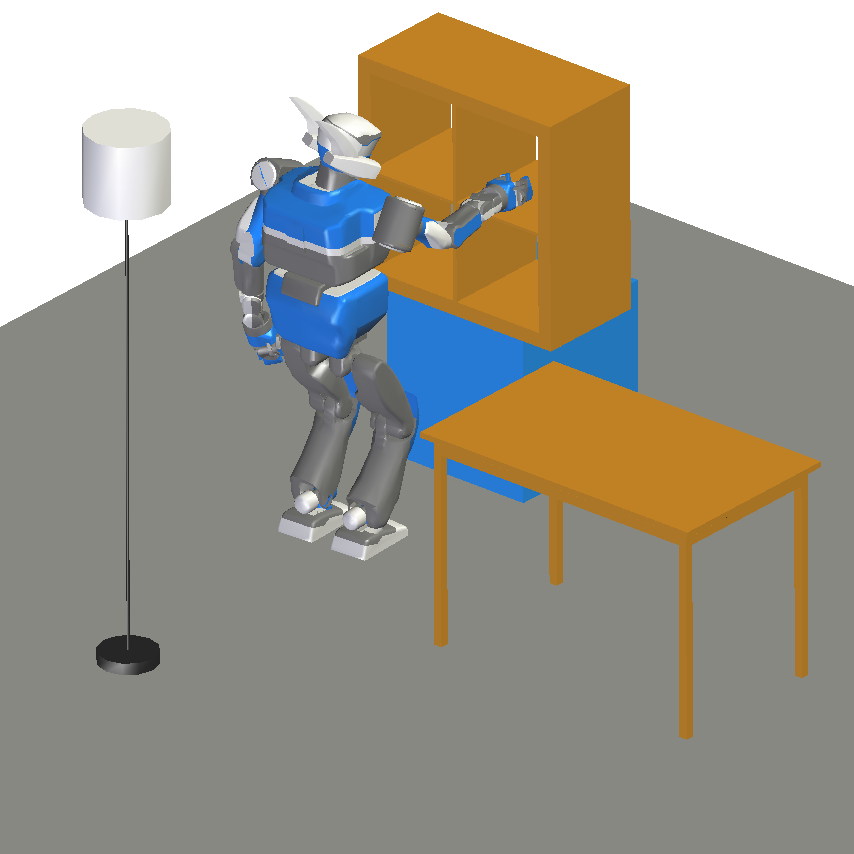
\includegraphics[width=\linewidth]{images/trajectory-8.png}
  \end{center}
  \caption{The HRP-2 robot drops a ball on a shelf while localizing
    itself using vision based localization. \label{fig:xp_setup_screenshot}}
\end{figure}


The experiment demonstrates that by localizing the robot while
walking, HRP-2 can reach a goal position independently of the
execution errors. In the chosen scenario, the robot must drop a ball
on a shelf after walking 2 meters. A more precise description of the
scenario is Fig.~\ref{fig:xp_setup_dim}. Empirically, we estimated the
HRP-2 mean drift to be around one centimeter per step. Considering
that 32 steps are required to reach the goal without hitting the
obstacles, the usual drift would prevent the task from being
accomplished.

\begin{figure}[ht!]
  \begin{center}
    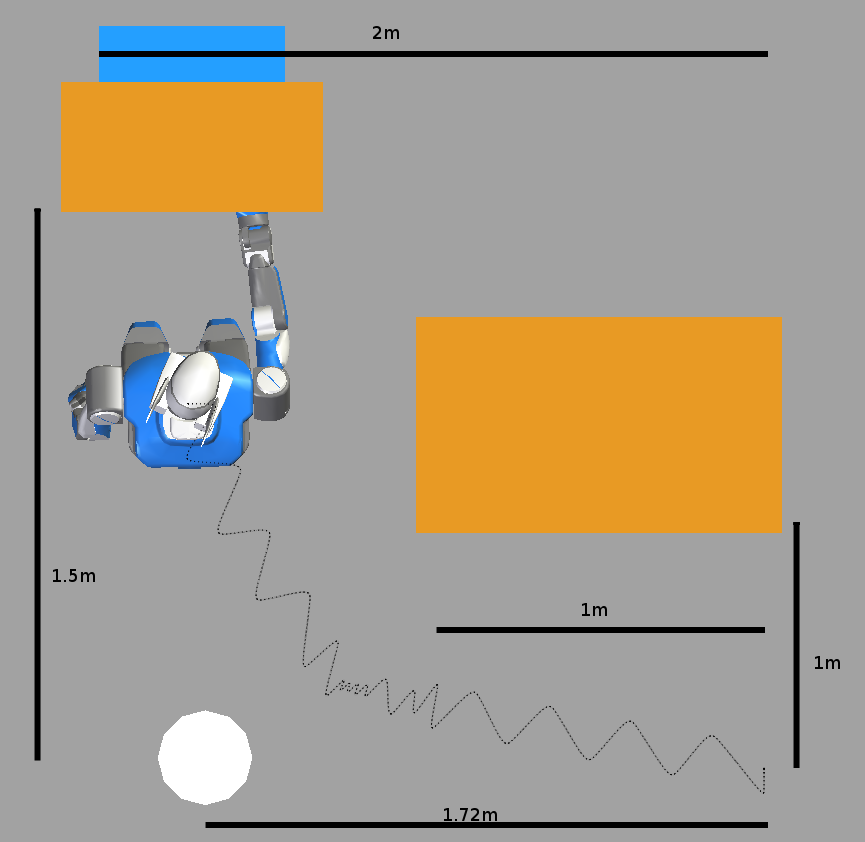
\includegraphics[width=\linewidth]{images/dimensions.png}
  \end{center}
  \caption{Experimental setup description (top view). The dotted line
    displays the robot waist trajectory.\label{fig:xp_setup_dim}}
\end{figure}


The camera trajectory estimated by the localization algorithm is
validated using motion capture data. Markers have been placed on both
the robot head (FIXME and left foot?) to provide ground truth.


Finally, the camera position is given by the algorithm described in
detail in the previous sections. During the experiments, the acquired
image resolution was $320 \times 240$. The localization module has
been running at a mean rate of 16\hertz~during the experiments. The
vision computer running the vision based localization node is a
Intel\textregistered Core\texttrademark\ 2 CPU T7200~@~2.00GHz with
2Gb.\ of RAM.


\subsection{Comparison to Motion Capture Data}\label{sec:mocap}

The Table.~\ref{tab:mocap_comparison} contains the camera position
estimated by the motion capture system and by the localization
algorithm. The mean error is FIXME meters and FIXME rad. Drop in the
algorithm precision can occur when the robot enters a part of the map
which is not dense enough or where the environment does not
incorporate enough texture to detect enough interest points.
%FIXME we will see depending on the final data...


The used motion capture system is a Motion Analysis system relying on
six Eagles and four Hawks cameras. It provides an estimation of the
camera position at 200\hertz~with a precision error of less than one
centimeter.

%FIXME write conclusion -> summarize results.

\begin{figure}[ht!]
  \begin{center}
    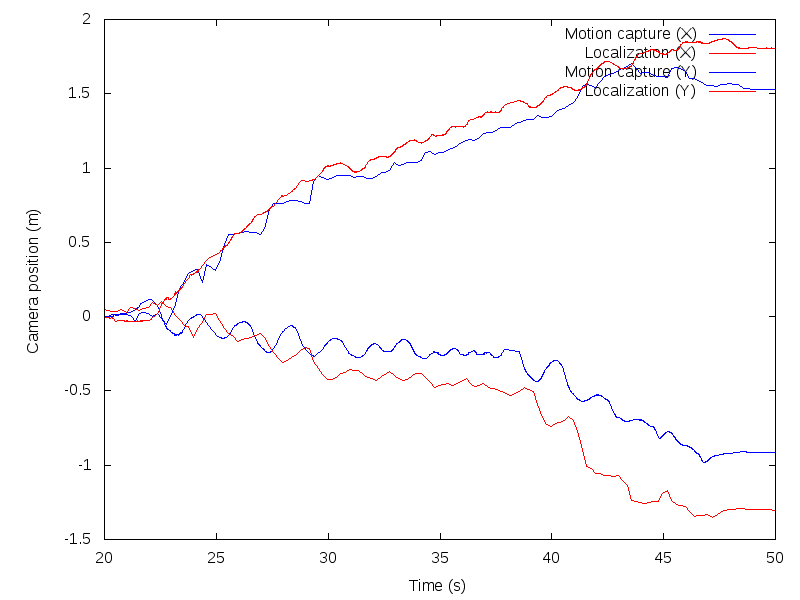
\includegraphics[width=\linewidth]{data/mocap.png}
  \end{center}
  \caption{Camera position estimated by both the motion capture system
    and the localization algorithm. \label{tab:mocap_comparison}}
\end{figure}

\subsection{Timing Evaluation}\label{sec:timing}
\PFA{Here there should be a table for timing evaluation, describing the mean computation times of the vision and control systems}
%%% Local Variables:
%%% ispell-local-dictionary: "american"
%%% LocalWords:  odometry HRP
%%% End:

\section{Future Work and Conclusions}\label{sec:conclusions}
In this article, we demonstrated that vision-based localization allows humanoid robots to achieve complex tasks. By integrating the vision algorithm into the control framework, we have been able to gradually
reshape the trajectory in order to compensate for execution errors. This allowed the robot to achieve complex tasks which would be difficult to realize otherwise.

However, several intesresting additions remain to be integrated. First, the local trajectory modifications are not checked to make sure that no auto-collision occurs. Currently, a conservative maximum correction (i.e.\ 2 centimeters\PFA{Again} every two steps) is imposed for safety. By applying recent works such as fast feasibility tests described by~\citet{Perrin10icra}, we would be able to increase the maximum correction without compromising the robot safety. Second, the HRP-2 robot embeds an Inertial Measurement Unit
which could be used to estimate the robot chest attitude. It would definitely be interesting to provide an initial estimation of the robot motion to help the localization process. In addition, we are interested in improving the capabilities of our visual SLAM and vision-based localization systems towards the goal of long-term localization to deal with possible changes in the environment.

\TM{Do we need more future work? / longer conclusion?}
\PFA{No, I think we are fine with that}
%%% Local Variables:
%%% ispell-local-dictionary: "american"
%%% LocalWords:  odometry HRP
%%% End:


\section*{Acknowledgments}

%% Use plainnat to work nicely with natbib.
\bibliographystyle{plainnat}
\bibliography{references}

\end{document}
